%=========================================================================
% (c) 2011, 2012 Josef Lusticky <xlusti00@stud.fit.vutbr.cz>

\chapter{NTP client in Contiki OS}
For implementation of a reasonably useful NTP client
operating system must be able to set, get
and eventually adjust time.
Apart from that, ability of communicating over UDP is also required.

Thanks to uIP, described in section~\ref{sec:contiki-uip}, communication is
not a matter for Contiki OS.
Contiki is also able to use Domain Name System for IPv4 address resolution.
DNS resolution of IPv6 addresses was not implemented in Contiki OS
at the time of writing~\cite{contiki-docs}.
The main problem of NTP client implementation for Contiki is therefore total
lack of real-time support.
Not only no common interface availability but also
almost no platform-specific code has been implemented towards time support yet.
Contiki provides basic clock interface particularly for use of timers though.
This interface is common for all supported platforms,
but the particular implementation is platform specific.

Another deal is possible packet loss if communication uses UDP on transport layer.
The reason this can happen often is explained in section~\ref{sec:contiki-uip}.

For developing and testing Contiki NTP client the AVR Raven platform with ATmega1284P~\cite{avr-datasheet} was used.
% do not mention, appendix?
How to get a working setup with Contiki on this platform is described in
%!%% CHECK THIS %%%
docs/setup.pdf file on the CD enclosed to this thesis.
%%% CHECK THIS %%%

\section{Required hardware clock interface}
Contiki features a basic clock interface with a simple goal - measuring time.
This interface provides needed calls for timers and its definition is to be found in {\it{/core/sys/clock.h}} file.
Specific implementations of this common interface are located in {\it{/cpu}} directory of Contiki source code.
The interface provides call for initialising CPU's clock system - {\it{clock\_init}}, that is automatically called during
boot sequence of Contiki.
The goal of the {\it{clock\_init}} call is to set up
appropriate counter registers and interrupt service routines. %! TODO .. as described in chapter..
On AVR CPU this call is implemented as C macro which evaluates to specific setup code for each CPU
when compiling.
The setup code is not common to all CPUs because of differences among them - e.g. there are usually
only three Timer/Counter modules, but AVR ATmega1284P has four Timer/Counter modules~\cite{avr-datasheet}.

%At least one of those is always 16 bit wide
%This extra module on AVR ATmega1284P is used for
% three vs. 3

%clock\_seconds
%CLOCK\_SECOND
This is however enough for implementing a reasonable time interface and using it for NTP client later.

% ntp interface extending the clock library, similar to posix calls

%!!AVR

Adjusting time - COMPARE\_REGISTER = 31 => 128Hz => 1s = 1s
FREQ = 32768/8 / 32
COMPARE\_REGISTER = 30 => ca132.129Hz => 1s = ca1.032258s
FREQ = 32768/8 / 31
COMPARE\_REGISTER = 32 => 124.12per => 1s = 0.96p
FREQ = 32768/8 / 33

=> fastest adjust is 0,03s / s


Each TCNT2 increment is $\frac{1}{128 \times 32} \doteq 0,000244$ s
2,44ms minimum clock slew
This is also minimal possible clock adjustment.


Adjustments will influence the timers.
Applications requiring ...TODO...
are therefore advised to use rtimers,
because they have its own clock module as described in section~\ref{sec:contiki-timers}.

%=========================================================================
% (c) 2011, 2012 Josef Lusticky

\section{Operating system time interface - TODO}
%Since there is no way of setting, getting and adjusting the time in Contiki OS,
%the interface for setting, getting and adjusting time was developed in this thesis.
New structure for expressing time values was implemented.
This structure is similar to POSIX {\it{timespec}} structure,
described in section~\ref{sec:others-posix}.
However, name was chosen {\it{time\_spec}} to avoid collision with
existing POSIX-compliant systems.
\begin{lstlisting}
struct time_spec {
  long sec;
  long nsec;
};
\end{lstlisting}
This structure consists of two signed long values for expressing seconds and nanoseconds.
The value 0 seconds and 0 nanoseconds is equal to Unix prime epoch (1st January 1970).
In case of seconds part, the 32-bit signed long value was chosen because
it can conveniently
represent real-time values as well as local clock adjustment values, which may also be negative.
%! The existing value {\it{seconds}}, representing uptime in Contiki, is of the unsigned long type.
Such time representation will wrap around in year 2038 and is facing
what is commonly known as the year 2038 problem~\cite{posix}.

In case of nanoseconds part, the 32-bit signed long value was chosen because
one second has 1~000~000~000 nanoseconds and it is
desirable to be able to express positive as well as negative values for local clock adjustments.
As 32-bit signed long type shall be able to express values from -$2^{31}$-1 (-2~147~483~647)
to $2^{31}$-1 (2~147~483~647)~\cite{c99},
such representation will therefore never wrap around.

It should be noted that signed long data type does not have to always result in a 32-bit variable -
it is up to compiler what data width it chooses for each data type.
But as ISO C99 standard states, the maximum value for an object of type signed long
shall be greater or equal $2^{31}$-1 (2~147~483~647)~\cite{c99}.
This in fact results in at least 32-bit variable unless the compilation setting is changed.
Next to this, as the already presented variable {\it{seconds}} is of unsigned long type,
the value {\it{sec}} in {\it{time\_spec}} structure %and {\it{boottime}}
shall be of the same data width as arithmetic operations are made on them.

Usage of unsigned data type delays the wrap around problem to year 2106,
however will disable use of negative values needed for adjusting local clock.
%As current NTP Era ends 2036 code has to be changed anyway...~\cite{ntp-y2k}.

Setting the current time is only possible within one second precision -
finer time setting must be made through time adjustments described further.
Implemented {\it{clock\_set\_time}} function computes when the system started
in seconds since the Epoch and saves the result in newly implemented {\it{boottime}} variable.

Not only no variables incremented every interrupt nor any internal clock registers
are affected, but also already presented variable {\it{seconds}} is not modified.
This variable, counting uptime in seconds,
is particularly used by stimers in Contiki
and modifying it would lead to misbehaviour of stimer library
described in section~\ref{sec:contiki-timers}.

Thanks to this newly implemented {\it{clock\_set\_time}} function and {\it{boottime}} variable,
running Contiki system is able to tell uptime, current time and
time when was the system booted.
\begin{lstlisting}
volatile unsigned long boottime;

void
clock_set_time(unsigned long sec)
{
  boottime = sec - seconds;
}
\end{lstlisting}

Getting the correct current time is only possible if it was set using
the {\it{clock\_set\_time}} function before.
Newly implemented function {\it{clock\_get\_time}} is then able to tell the
current time in seconds since the Epoch by simply adding {\it{boottime}},
and {\it{seconds}}.
%! TODO
Nanoseconds part is filled using {\it{scount}} variable counting number of
interrupts within a second.
Since this variable is incremented every interrupt and there are {\it{CLOCK\_SECOND}} interrupts
per second, it is possible to get resolution of $\frac{1~000~000~000}{CLOCK\_SECOND}$ ns.
The same resolution have Contiki timers, described in section~\ref{sec:contiki-timers}.
\begin{lstlisting}
void
clock_get_time(struct time_spec *ts)
{
  ts->sec = boottime + seconds;
  ts->nsec = (1000000000 / CLOCK_SECOND) * scount;
}
\end{lstlisting}
Because {\it{1000000000}} and {\it{CLOCK\_SECOND}} are both constants, the compiler is able to
calculate the result of division during compile time.
Furthermore as both numbers are integers, the result is integer as well~\cite{c99}.
The most of CPU time is therefore spent on multiplication.
E.g. if the code is compiled using GCC version 4.3.5,
multiplication of two 32-bit variables takes 33 instructions including {\it{call}} and {\it{ret}}
instructions for entering and returning from the {\it{\_\_mulsi3}} routine, which computes
the result of multiplication.
%avr-objdump
According to AVR Instruction Set manual~\cite{avr-instruction-set},
this results in 48 clock cycles overhead,
which takes 3~000 nanoseconds assuming 16MHz CPU clock.
The timestamp provided is therefore not exact.
However, since this consumed time strongly depends on architecture and compiler specifications,
no correction was implemented to remove this inaccuracy.
The application must be instead aware that the timestamp is not exactly accurate.

TODO: Greater precision is further implemented by reading counter register.

TODO: Adjust time
POSIX:
Time values that are between two consecutive non-negative integer multiples
of the resolution of the specified clock are truncated down to the smaller multiple of the resolution.


\section{NTP client implementation}
Structures representing NTP message were borrowed from OpenNTPD NTP Unix daemon.
%They are not using the GCC extension for representing a bit field.

Packet sanity tests~\cite{ntp-arch}.

A client sends messages to each server with a poll interval of $2^{\tau}$
seconds, as determined by the poll exponent $\tau$ (tau).
In NTPv4, $\tau$ ranges from 4 (16 s) to 17 (36 h).


% filling the packet
Precision express strictly speaking elapsed time to read the system clock from userland~\cite{ntp-arch}.
However most implementation supply clock precision.
%Dragonfly BSD:
%wmsg.precision = -6;
%Chrony, NTP.org - getting resolution, gettimeofday, clock_getres
\begin{lstlisting}
// set clock precision - convert Hz to log2 - borrowed from OpenNTPD
int b = CLOCK_SECOND; // CLOCK_SECOND * OCR2A
int a;
for (a = 0; b > 1; a--, b >>= 1)
  {}
msg.precision = a;
\end{lstlisting}
This will work for clock precision greater or equal 1s, i.e. CLOCK\_SECOND must be greater or equal 1.
%refer to CLOCK\_SECOND - is always greater or equal 1

The clock are set if the time difference is greater than XX seconds. %! TODO
\begin{lstlisting}
if (labs((signed long) (ts.sec - tmpts.sec)) > 2)
{
  clock_set_time(ts.sec);
}
\end{lstlisting}
Even if {\it{tmpts.sec}} value is greater than {\it{ts.sec}} value,
subtracting and casting to signed type gives correct (negative) result~\cite{c99}.
Assuming 32-bit data types this will work until 2038 when wrap around can occur due to difference
between {\it{ts.sec}} and {\it{tmpts.sec}} greater than $2^{31}$-1 (2~147~483~647).
But as NTP Era 0 ends 2036 the NTP client code must be changed in the future anyway.

%! TODO

%Adjusting time
%1/128/32 = 0.000244141
%0.000244141x32x127+0.000244141x31 == smallest possible adjustment == 244us

\section{NTP values and converts}
Unlike the RFC 5905~\cite{rfc5905} shows, there are no 64 bit values. %! RFC - A.4. Kernel System Clock Interface
No floating point numbers - library.
Division of unsigned integer number by 2 is automatically translated by compiler to logical right shift,
making it fast operation.

Converting between NTP and local timestamps requires floating point unit or 64-bit numbers.
according to output from avr-size tool, using 64-int number for conversion
uses 4~330 bytes more in program section of resulted binary file 
and simulated floating point operation takes 3~474 bytes more
than algorithm developed?

%
% NEGATIVE result for the first time
In some scenarios where the initial frequency offset of the client is
  relatively large and the actual propagation time small, it is
   possible for the delay computation to become negative.  For instance,
   if the frequency difference is 100 ppm and the interval T4-T1 is 64
   s, the apparent delay is -6.4 ms.  Since negative values are
   misleading in subsequent computations, the value of delta should be
   clamped not less than s.rho, where s.rho is the system precision
   described in Section 11.1, expressed in seconds~\cite{rfc5905}.
%

\section{Network communication}
% IEEE 802.15.4
as RFC~4944 written by 6lowpan working group of IETF
made the underlaying IEEE 802.15.4 layer
look like an IPv6 link~\cite{6lowpan} and
\begin{figure}
  \centering
  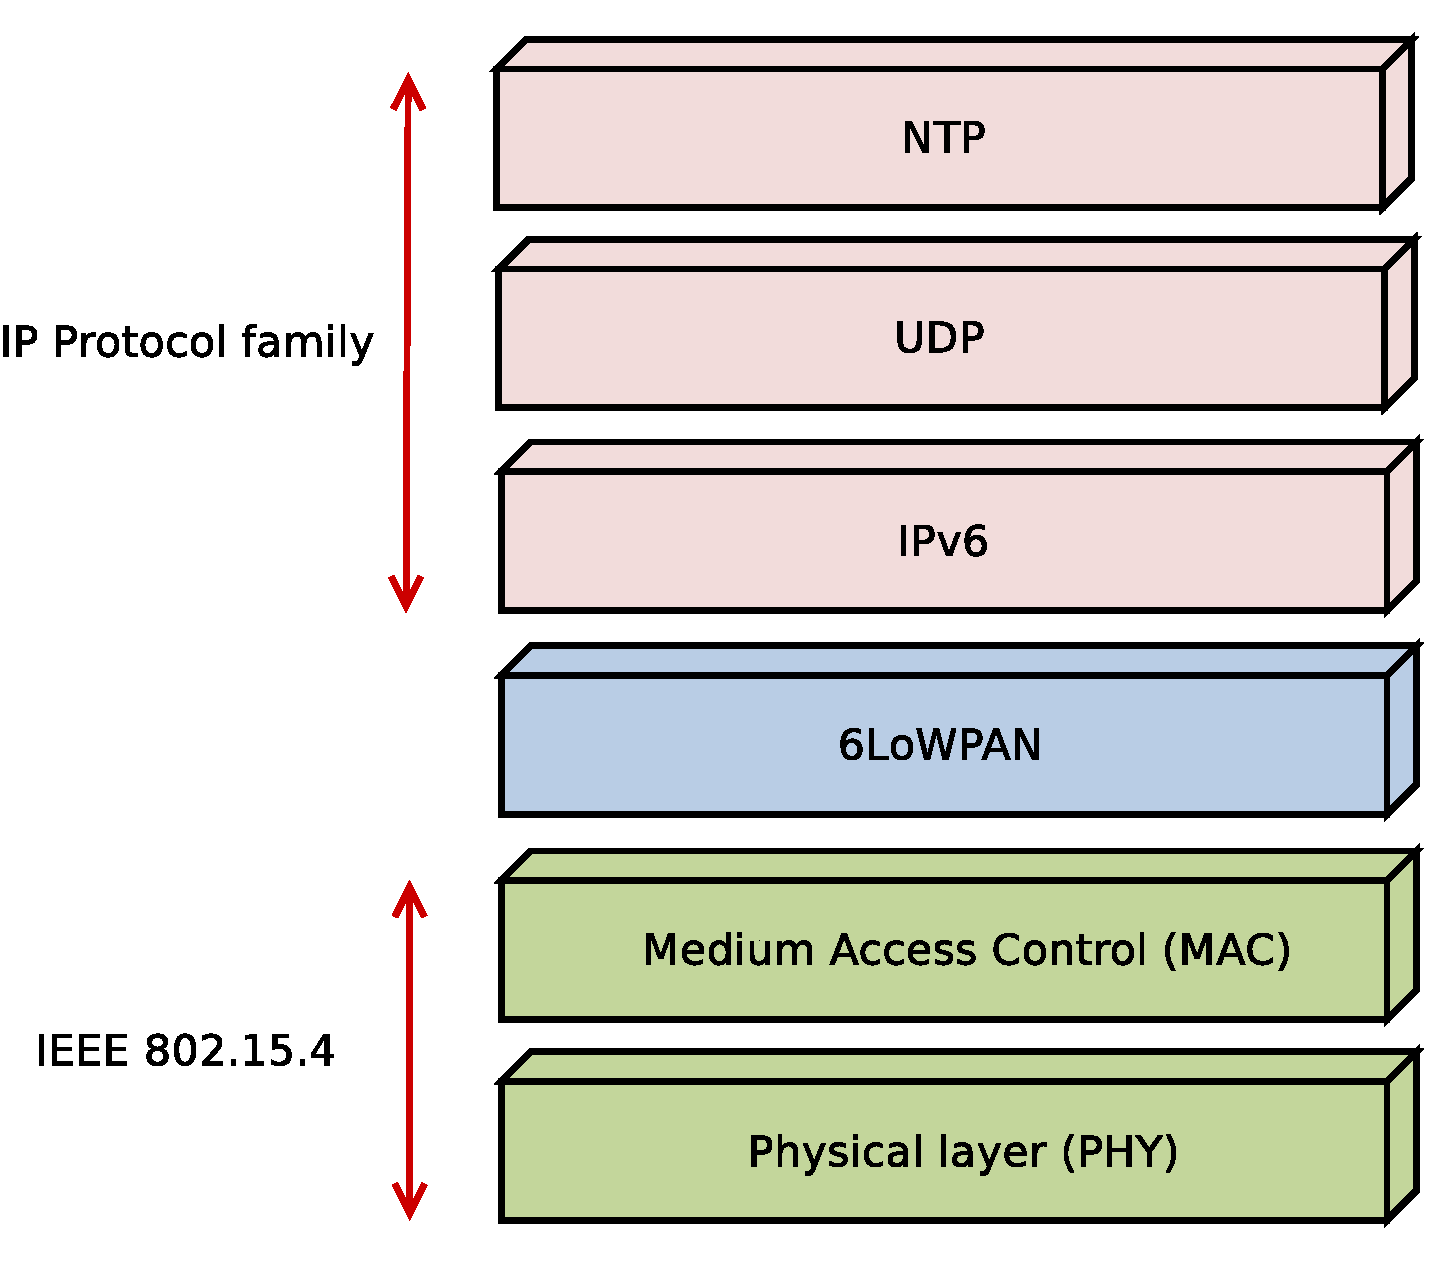
\includegraphics[width=9cm,keepaspectratio]{fig/6lowpan.pdf}
  \caption{Communication stack with 6lowpan layer}
  \label{fig:implementation-6lowpan}
  \bigskip
\end{figure}

NTP server can be specified in Makefile or
during compilate time using {\it{REMOTE\_HOST}} define.
%! TODO
TODO: If no host is specified,
NTP client assumes NTP broadcast communication mode.


% There is no IPv4 support...

%The uIP packet buffer is accessed through
%the uip\_buf array and is used to hold incoming and outgoing packets.
%The device driver should place incoming data into this buffer.
%When sending data, the device driver should read the link
%level headers and the TCP/IP headers from this buffer.
%The size of the link level headers is configured by the UIP\_LLH\_LEN
%define and in case of ethernet it is 14.

%The application data need not be placed in this buffer, so
%the device driver must read it from the place pointed to by the
%uip\_appdata pointer %as illustrated by the following example:
